% =====================================================================
%  fbd_uniaxial.tex -- the manual's figure of chapter 2 (One-dimensional
%  continuum mechanics). Drawn from the ME 697 Unit 3 sheet's figure
%  (Equation_Sheets/Unit_03_rev-1/fbd_uniaxial.tex, D. E. Kittell), which stays
%  the sheet's; this copy is the manual's. Built by 'make manual'.
% =====================================================================
\documentclass[tikz,border=10pt]{standalone}
\usetikzlibrary{arrows.meta}

% ---- Muted academic theme ----
\definecolor{slate}{HTML}{2C3E50}
\definecolor{oiblue}{HTML}{0072B2}
\definecolor{oivermil}{HTML}{D55E00}
\definecolor{oigreen}{HTML}{009E73}

\tikzset{
  elem/.style   = {draw=slate, thick, fill=oiblue!15},
  stress/.style = {-{Stealth[length=8pt, width=6pt]}, oivermil,
                   line width=1.4pt},
  dim/.style    = {{Straight Barb[length=5pt]}-{Straight Barb[length=5pt]},
                   slate, thin},
  ext/.style    = {slate, thin, densely dashed},
  flow/.style   = {-{Stealth[length=7pt, width=5.5pt]}, oigreen,
                   line width=1.2pt},
  axis/.style   = {-{Stealth[length=5pt]}, slate, thin},
}

\begin{document}
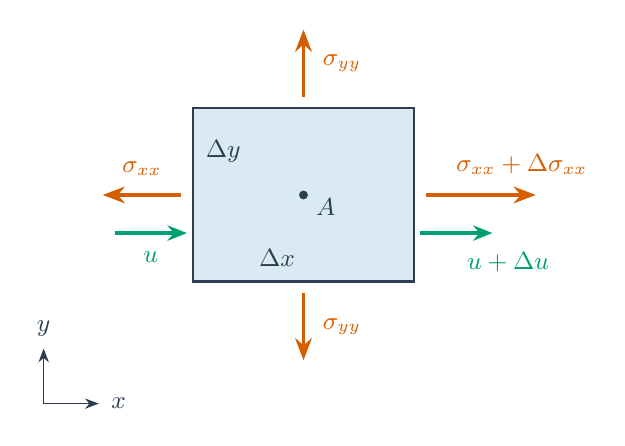
\begin{tikzpicture}[font=\sffamily, text=slate]
  \def\W{2.8}   % Delta x
  \def\H{2.2}   % Delta y
  \def\cx{0.5*\W}
  \def\cy{0.5*\H}

  % element
  \draw[elem] (0,0) rectangle (\W,\H);

  % center dot, area A
  \fill[slate] (\cx,\cy) circle (1.6pt);
  \node[below right=1pt, font=\small] at (\cx,\cy+0.05*\H) {$A$};

  % ---- stresses (tension positive: arrows outward) ----
  % left face: sigma_xx
  \draw[stress] (-0.15,\cy) -- (-1.15,\cy)
      node[midway, above=3pt, text=oivermil, font=\small] {$\sigma_{xx}$};
  % right face: sigma_xx + Delta sigma_xx (slightly longer)
  \draw[stress] (\W+0.15,\cy) -- (\W+1.55,\cy)
      node[anchor=south west, text=oivermil, font=\small]
      at (\W+0.40, \cy+0.12) {$\sigma_{xx}+\Delta\sigma_{xx}$};
  % top face: sigma_yy
  \draw[stress] (\cx,\H+0.15) -- (\cx,\H+1.0)
      node[midway, right=3pt, text=oivermil, font=\small] {$\sigma_{yy}$};
  % bottom face: sigma_yy (no increment)
  \draw[stress] (\cx,-0.15) -- (\cx,-1.0)
      node[midway, right=3pt, text=oivermil, font=\small] {$\sigma_{yy}$};

  % ---- mass flow / velocity (energy: stress power, mass flux) ----
  \draw[flow] (-1.0, 0.28*\H) -- (-0.08, 0.28*\H)
      node[midway, below=3pt, text=oigreen, font=\small] {$u$};
  \draw[flow] (\W+0.08, 0.28*\H) -- (\W+1.0, 0.28*\H)
      node[pos=0.5, below=3pt, anchor=north west, text=oigreen, font=\small]
      at (\W+0.05, 0.28*\H) {$u+\Delta u$};

  % ---- edge dimensions (directly on edges) ----
  \node[above=2pt, font=\small] at (0.38*\W, 0) {$\Delta x$};
  \node[font=\small] at (0.38, 0.75*\H) {$\Delta y$};

  % ---- x-y fiducial ----
  \begin{scope}[shift={(-1.9,-1.55)}]
    \draw[axis] (0,0) -- (0.7,0) node[right=1pt, font=\small] {$x$};
    \draw[axis] (0,0) -- (0,0.7) node[above=1pt, font=\small] {$y$};
  \end{scope}
\end{tikzpicture}
\end{document}
